%
% CHAPTER Versuch 2
%
\chapter{Abtasttheorem}
Das Abtasttheorem besagt, dass ein auf $fmax$ bandbegrenztes Signal mit einer Frequenz von größer 2 \cdot $fmax$ abgetastet werden muss, damit man es aus dem zeitdiskreten Signal wieder exakt rekonstruieren kann.
In diesem versuch werden wir unser Signal bis hin zur Abtastfrequenz erhöhen um zu sehen, was dies für auswirkungen hat.
\label{chap:Abtasttheorem}
\section{Fragestellung, Messprinzip, Aufbau, Messmittel}
\label{chap:VERSUCH_5_FRAGESTELLUNG}
Die Abtastfrequenz unseren AD-Wandlers beträgt 80000$Hz$. Die Nyquistfrequenz beträgt somit genau 4$kHz$.
Angefangen von der halben Nyquistfrequenz bis zur doppelten variieren wir die Frequenz eines Sinusgenerators in 7 schritten, die daugehörige Foriertransformierte wird in den folgenden Bildern gezeigt:
\section{Ergebnis}
\label{chap:VERSUCH_5_MESSWERTE}

\begin{figure}[H]
\centering
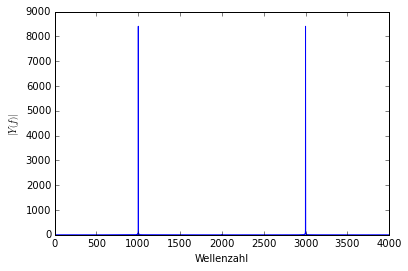
\includegraphics[width=0.75\textwidth]{5_2000.png}
\caption{Frequenzbereich 2kHz}
\label{fig:F2}
\end{figure}
\begin{figure}[H]
\centering
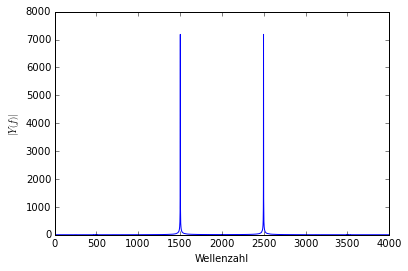
\includegraphics[width=0.75\textwidth]{5_3000.png}
\caption{Frequenzbereich 3kHz}
\label{fig:F3}
\end{figure}
\begin{figure}[H]
\centering
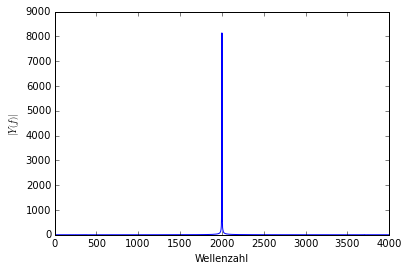
\includegraphics[width=0.75\textwidth]{5_4000.png}
\caption{Frequenzbereich 4kHz}
\label{fig:F4}
\end{figure}
\begin{figure}[H]
\centering
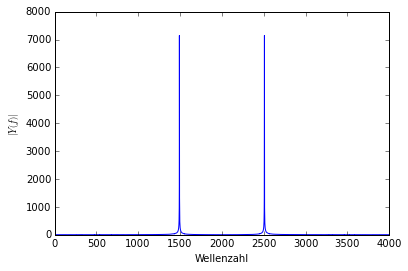
\includegraphics[width=0.75\textwidth]{5_5000.png}
\caption{Frequenzbereich 5kHz}
\label{fig:F5}
\end{figure}
\begin{figure}[H]
\centering
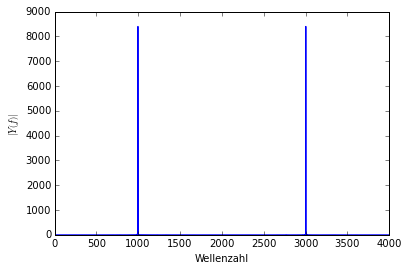
\includegraphics[width=0.75\textwidth]{5_6000.png}
\caption{Frequenzbereich 6kHz}
\label{fig:F6}
\end{figure}
\begin{figure}[H]
\centering
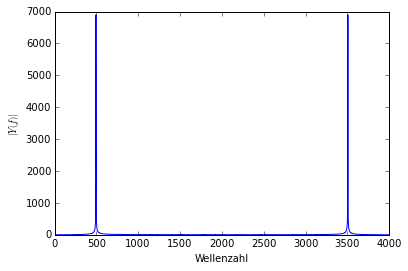
\includegraphics[width=0.75\textwidth]{5_7000.png}
\caption{Frequenzbereich 7kHz}
\label{fig:F7}
\end{figure}
\begin{figure}[H]
\centering
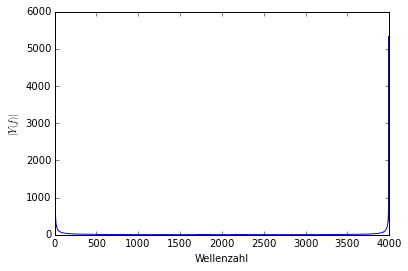
\includegraphics[width=0.75\textwidth]{5_8000.png}
\caption{Frequenzbereich 8kHz}
\label{fig:F8}
\end{figure}


\section{Auswertung und Interpretation}
\label{chap:AUSWERTUNGUNDINTERPRETATION5}
Wir erkennen, dass sich im Frequenzbereich zwei Piks aufeinander zu bewegen, bei der Nyquistfrequenz liegen diese Piks sogar genau übereinander. Wird die Frequenz noch weiter erhöht, erkennen wir, dass sich die Peeks wieder ausseinander bewegen, bi sie bei der abtastfrequenz (8000$Hz$) kaum mehr erkennbar sind. im Zeitbereich sollte hier, falls die frequenz exakt getroffen wurde eine Konstante angezeigt werden. Dies war in unserem Beispiel allerdings nicht der fall, wir lagen minimal daneben, was aber für diesen Versuch kein Problem darstellt.